\chapter{Teorías de la velocidad de reacción}\label{ch:b3:rate-theories}

En 2017 se aprobó un medicamento cuya única diferencia con otro más antiguo es
que los seis átomos de hidrógeno de sus dos grupos metoxi son átomos de deuterio. El
hígado degrada el fármaco cortando exactamente esos enlaces C--H, y un enlace C--D
se corta varias veces más despacio: la molécula pesada permanece más tiempo en la
sangre y se toma en dosis menores y menos frecuentes. Nada en la ley de
Arrhenius explica por qué un neutrón en un núcleo habría de frenar una reacción. Este
capítulo deduce las constantes de velocidad a partir de las propiedades moleculares: primero a partir de las
colisiones, después a partir de la forma de la \omterm{def:b3:computational-chemistry:pes}{superficie de energía potencial} y de las
funciones de partición de la \omterm{def:b3:rate-theories:tst}{teoría del estado de transición}, que predice la magnitud de
esos efectos isotópicos; termina con las reacciones en disolución, en las que el disolvente
impone un límite de velocidad.

\begin{recall}
El volumen del primer año definió la constante de velocidad, la ley de Arrhenius $k =
A\eu^{-E_a/RT}$ con su energía de activación y su factor preexponencial, las etapas
elementales, el estado de transición, el perfil energético a lo largo de la coordenada de reacción
y el postulado de Hammond. El volumen del segundo año definió la fuerza iónica y los coeficientes
de actividad, con la ley límite de Debye--Hückel $\log\gamma_i = -Az_i^2\sqrt I$ ($A \approx
0.51$ en agua a \qty{25}{\celsius}), y ajustó rectas por mínimos cuadrados.
El \cref{ch:b3:computational-chemistry} introdujo las \omterm{def:b3:computational-chemistry:pes}{superficies de energía potencial};
los \cref{ch:b3:partition-functions,ch:b3:statistical-thermo-applied} calcularon
constantes de equilibrio a partir de funciones de partición y de \omterm{def:b3:quantum-model-systems:oscillator}{energías de punto cero}. De la
física: la distribución de Maxwell--Boltzmann de las velocidades moleculares y la ley de Fick
de la difusión.
\end{recall}

\begin{omfigure}
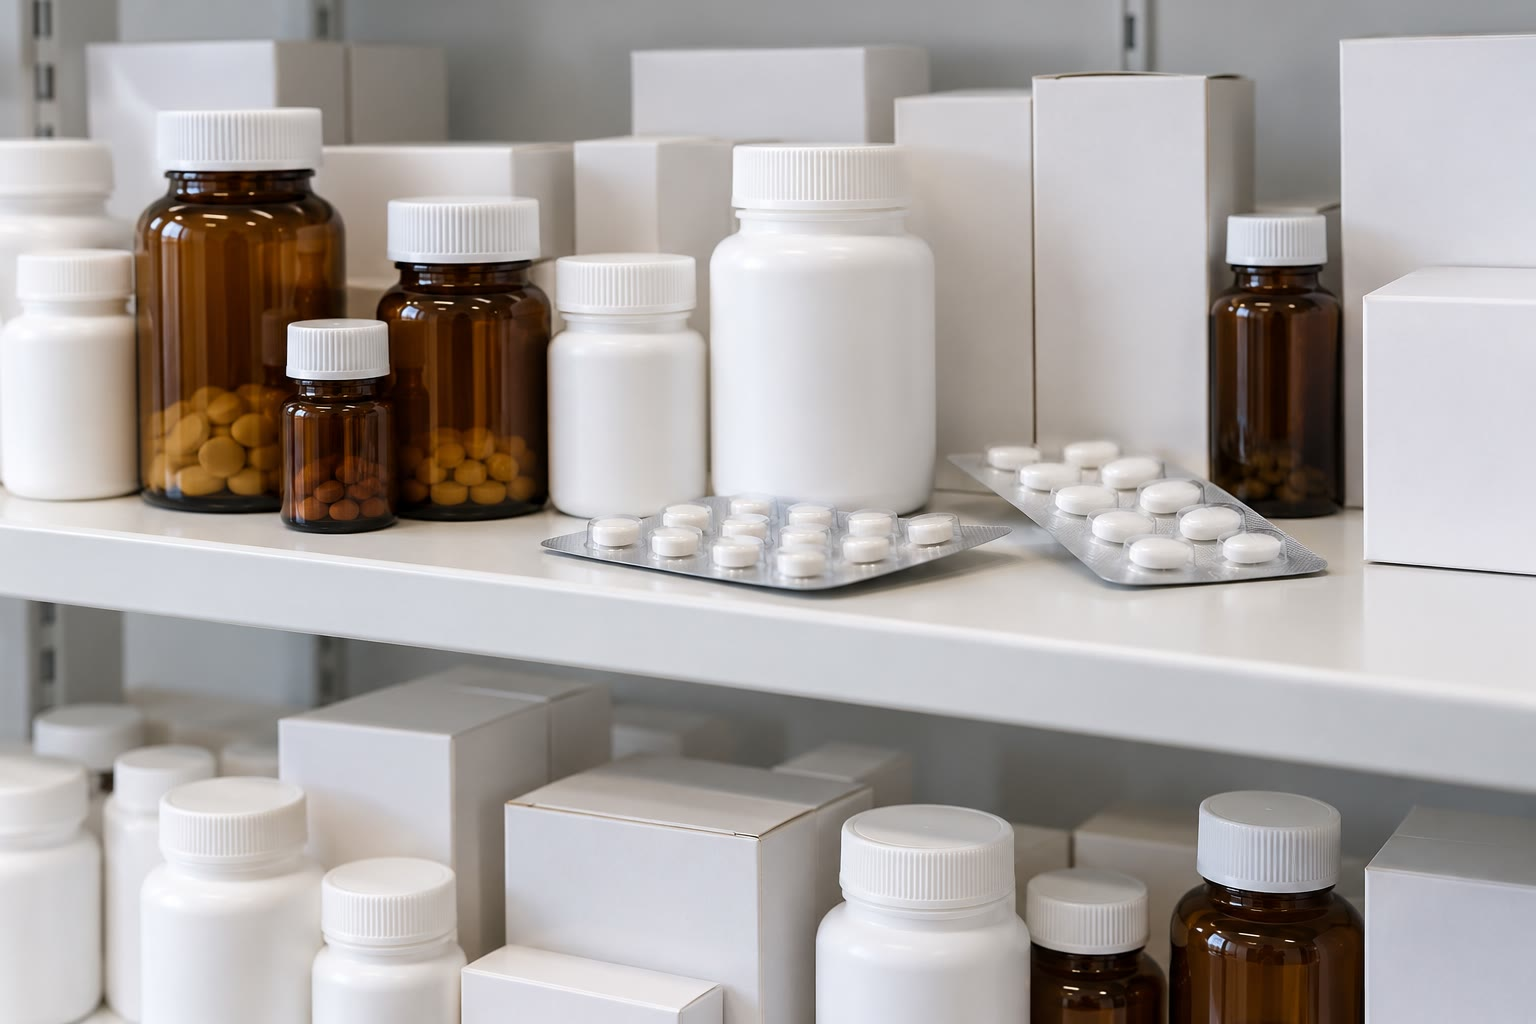
\includegraphics[width=0.6\linewidth]{images/book4/ai/b3-12-pharmacy.jpg}

{\small Medicamentos en el estante de una farmacia. Sustituir el hidrógeno por deuterio en los
enlaces que el hígado ataca primero puede alargar el tiempo que un fármaco permanece en el organismo.}
\end{omfigure}

\section{Teoría de las colisiones}

Dos moléculas de un gas solo pueden reaccionar si se encuentran. Se modelizan como esferas duras
de diámetros $d_{\mathrm A}$ y $d_{\mathrm B}$: chocan cuando sus centros pasan a menos de $d =
\frac12(d_{\mathrm A} + d_{\mathrm B})$ uno del otro.

\begin{definition}[Sección eficaz de colisión, factor estérico]\label{def:b3:rate-theories:collision}
La \emph{sección eficaz de colisión}\index{seccion eficaz de colision@sección eficaz de colisión} de dos moléculas
es el área $\sigma = \pi d^2$ del disco, perpendicular a su velocidad relativa,
por cuyo interior debe pasar el centro de una para que choque con la otra. El
\emph{factor estérico}\index{factor esterico@factor estérico} $P$ es la razón entre el factor
preexponencial medido de una reacción y el que predice la teoría de las colisiones.
\end{definition}

\begin{omfigure}
\begin{tikzpicture}[font=\small, >=Stealth]
  \shade[ball color=omDef!40] (0,0) circle (0.45);
  \node at (0,0) {A};
  \draw[black!50, dashed] (-0.0,0.85) -- (5.2,0.85) (-0.0,-0.85) -- (5.2,-0.85);
  \draw[black!60] (0,0) ellipse (0.25 and 0.85);
  \draw[<->] (-0.45,0) -- (-0.45,0.85) node[midway, left] {$d$};
  \shade[ball color=omThm!40] (3.3,0.55) circle (0.4);
  \node at (3.3,0.55) {B};
  \shade[ball color=omThm!20] (4.6,1.45) circle (0.4);
  \node at (4.6,1.45) {B};
  \draw[->, thick] (0.6,0) -- (2.2,0) node[midway, below] {$v_{\mathrm{rel}}\,\Delta t$};
  \node[anchor=west, align=left, font=\scriptsize] at (5.3,0) {cilindro de\\ sección\\ $\sigma = \pi d^2$};
  \node[font=\scriptsize, anchor=south] at (3.3,1.0) {choca};
  \node[font=\scriptsize, anchor=south] at (4.6,1.9) {no choca};
\end{tikzpicture}

{\small El cilindro de colisión. Moviéndose a la velocidad relativa $v_{\mathrm{rel}}$, la molécula A barre
en un tiempo $\Delta t$ un cilindro de sección $\sigma = \pi d^2$, con $d$ la suma de los dos
radios; choca con toda molécula B cuyo centro esté dentro.}
\end{omfigure}

\begin{theorem}[Constante de velocidad de la teoría de las colisiones]\label{thm:b3:rate-theories:collision}
Si toda colisión cuya energía cinética según la línea de los centros supera un
umbral $E_0$ (por mol) conduce a reacción, la constante de velocidad de $\mathrm{A + B} \to$
productos es
\[
  k = \sigma\bar v_{\mathrm{rel}}N_A\,\eu^{-E_0/RT}, \qquad \bar v_{\mathrm{rel}} = \sqrt{\frac{8kT}{\pi\mu}},\
  \mu = \frac{m_{\mathrm A}m_{\mathrm B}}{m_{\mathrm A} + m_{\mathrm B}} .
\]
\end{theorem}

\begin{proof}[Demostración parcial]
En un tiempo $\Delta t$, una molécula A barre un volumen $\sigma v_{\mathrm{rel}}\Delta t$ y choca con las
$n_{\mathrm B}\sigma v_{\mathrm{rel}}\Delta t$ moléculas B que contiene: la frecuencia de colisiones por unidad de volumen
es $\sigma\bar v_{\mathrm{rel}}n_{\mathrm A}n_{\mathrm B}$, con $\bar v_{\mathrm{rel}}$ la velocidad relativa media dada por la
distribución de Maxwell--Boltzmann (que se admite de la física, con la \omterm{def:b3:quantum-model-systems:oscillator}{masa
reducida}). Ponderar cada colisión por su velocidad y conservar aquellas cuya energía
según la línea de los centros supera el umbral deja la fracción
$\eu^{-E_0/RT}$ de la frecuencia de colisiones (la integración sobre el parámetro de impacto se
admite). Convertir las densidades numéricas en concentraciones molares multiplica por
$N_A$.
\end{proof}

Como $\bar v_{\mathrm{rel}} \propto \sqrt T$, la energía de activación $E_a = RT^2\,\dd\ln k/\dd T$ vale $E_0 + \frac12RT$,
próxima al umbral. El factor preexponencial es del orden de
$10^{11}$~\unit{L.mol^{-1}.s^{-1}} para las moléculas pequeñas. Los factores medidos suelen ser
mucho menores: $P \ll 1$ para las moléculas que deben encontrarse con una orientación
particular, y la sección eficaz no tiene un valor único para las moléculas reales,
que no son esferas duras. La teoría de las colisiones da el orden de magnitud y
la dependencia con la temperatura; no puede dar $E_0$, que requiere la \omterm{def:b3:computational-chemistry:pes}{superficie de
energía potencial}.

\section{Superficies de energía potencial}

La reacción $\mathrm{H_A + H_BH_C \to H_AH_B + H_C}$ es la más sencilla que existe. Para una
aproximación colineal, la energía depende de dos distancias, $r_{\mathrm{AB}}$ y $r_{\mathrm{BC}}$, y puede dibujarse
como un mapa.

\begin{definition}[Punto de silla, camino de energía mínima]\label{def:b3:rate-theories:saddle}
Un \emph{punto de silla}\index{punto de silla} de una \omterm{def:b3:computational-chemistry:pes}{superficie de energía potencial} es un punto
en el que el gradiente se anula y la energía es máxima en una dirección y
mínima en todas las demás. El \emph{camino de energía mínima}\index{camino de energia minima@camino de energía mínima}
es el camino de máxima pendiente que baja del punto de silla a los valles de los reactivos
y de los productos; su longitud medida a lo largo de él es la coordenada de reacción,
y el punto de silla es el estado de transición.
\end{definition}

\begin{omfigure}
\begin{tikzpicture}
\begin{axis}[ompes, width=0.62\linewidth, xmin=0.4, xmax=3.0, ymin=0.4, ymax=3.0,
  xlabel={$r_{\mathrm{AB}}$ / \AA}, ylabel={$r_{\mathrm{BC}}$ / \AA},
  colorbar, colorbar style={ylabel={$E$ / eV}, ylabel style={font=\small},
  yticklabel style={font=\small}}, point meta min=-4.7, point meta max=-0.8]
\addplot3[contour prepared={labels=false}, thick] table {figdata/out/bachelor-3-pes-collinear-contours.dat};
\addplot3[ompath] table[x=x, y=y, z expr=0] {figdata/out/bachelor-3-pes-collinear-mep.dat};
\node[omsaddle] at (axis cs:0.918,0.918,0) {};
\node[font=\small, anchor=south west] at (axis cs:0.95,0.95,0) {silla};
\node[font=\small, anchor=west, fill=white, fill opacity=0.85, text opacity=1, inner sep=1.5pt] at (axis cs:2.05,1.0,0) {$\mathrm{H_A + H_BH_C}$};
\node[font=\small, anchor=west, fill=white, fill opacity=0.85, text opacity=1, inner sep=1.5pt] at (axis cs:0.95,2.55,0) {$\mathrm{H_AH_B + H_C}$};
\node[font=\small, anchor=north east] at (axis cs:2.95,2.95,0) {$\ce{H + H + H}$};
\end{axis}
\end{tikzpicture}

{\small Una \omterm{def:b3:computational-chemistry:pes}{superficie de energía potencial} modelo para $\ce{H + H2}$ colineal (forma LEPS construida
a partir de la curva de Morse de \ce{H2}, con un parámetro de Sato de 0.17 elegido como constante
del modelo). Curvas de nivel de \qty{-4.65}{eV} a \qty{-0.8}{eV}, con el cero de energía para tres átomos separados;
los valles están a \qty{-4.75}{eV}, la profundidad del pozo de \ce{H2}. En trazo discontinuo: el \omterm{def:b3:rate-theories:saddle}{camino
de energía mínima}, que cruza el \omterm{def:b3:rate-theories:saddle}{punto de silla} simétrico en $r_{\mathrm{AB}} = r_{\mathrm{BC}} = \qty{0.92}{\angstrom}$,
\qty{0.27}{eV} por encima de los valles en este modelo.}
\end{omfigure}

El camino sale del valle de los reactivos, donde $r_{\mathrm{BC}}$ se mantiene cerca de la longitud de enlace
de \ce{H2} mientras A se acerca, cruza el \omterm{def:b3:rate-theories:saddle}{punto de silla} y desciende al valle de
los productos. En el \omterm{def:b3:rate-theories:saddle}{punto de silla}, ambos enlaces están estirados hasta \qty{0.92}{\angstrom}: el enlace
antiguo está medio roto y el nuevo medio formado, y el coste energético de este
compromiso es la barrera. Para la reacción simétrica, el \omterm{def:b3:rate-theories:saddle}{punto de silla} está sobre la
diagonal; para una reacción exotérmica se desplaza hacia el valle de los reactivos (una
barrera temprana, un estado de transición parecido a los reactivos, como dice el postulado de
Hammond), y para una endotérmica, hacia el valle de los productos (una barrera tardía).
La posición decide qué energía ayuda: la energía de traslación, dirigida según
el valle de entrada, lleva a las moléculas por encima de una barrera temprana; una barrera
tardía, tras un recodo, se cruza más fácilmente con energía de vibración en el
enlace que se rompe. Son las reglas de Polanyi, confirmadas por experimentos de
haces moleculares.

\section{Teoría del estado de transición}

\begin{definition}[Complejo activado]\label{def:b3:rate-theories:activated-complex}
El \emph{complejo activado}\index{complejo activado} de una etapa elemental es el
conjunto de las configuraciones del sistema reaccionante situadas en una fina rebanada en torno al
\omterm{def:b3:rate-theories:saddle}{punto de silla}, perpendicular al \omterm{def:b3:rate-theories:saddle}{camino de energía mínima}; se trata como una
especie $\ce{AB^{\ddagger}}$, con su propia función de partición.
\end{definition}

\begin{definition}[Teoría del estado de transición, coeficiente de transmisión]\label{def:b3:rate-theories:tst}
La \emph{teoría del estado de transición}\index{teoria del estado de transicion@teoría del estado de transición} supone que los
\omterm{def:b3:rate-theories:activated-complex}{complejos activados} están en equilibrio con los reactivos, que todo complejo
que cruza la región del \omterm{def:b3:rate-theories:saddle}{punto de silla} hacia los productos acaba formándolos y que
el movimiento a lo largo de la coordenada de reacción es una traslación libre. El
\emph{coeficiente de transmisión}\index{coeficiente de transmision@coeficiente de transmisión} $\kappa \le 1$ corrige
los complejos que vuelven a cruzar hacia los reactivos.
\end{definition}

\begin{theorem}[Ecuación de Eyring]\label{thm:b3:rate-theories:eyring}
Para una etapa elemental $\mathrm{A + B} \to \mathrm{AB}^{\ddagger} \to$ productos,
\[
  k = \kappa\frac{k_BT}{h}\overline{K}{}^{\ddagger}, \qquad
  \overline{K}{}^{\ddagger} = \frac{\bar q^{\ddagger}/N_A}{(q_{\mathrm A}/N_A)(q_{\mathrm B}/N_A)}\,\eu^{-\Delta E_0^{\ddagger}/RT},
\]
donde $\bar q^{\ddagger}$ es la función de partición del \omterm{def:b3:rate-theories:activated-complex}{complejo activado} sin el
movimiento según la coordenada de reacción, las $q$ son funciones de partición molares por unidad
de volumen, y $\Delta E_0^{\ddagger}$ es la altura del nivel de punto cero del complejo por encima del
de los reactivos. En forma termodinámica, con $c^\circ = \qty{1}{mol/L}$ y la
molecularidad $m$,
\[
  k = \kappa\frac{k_BT}{h}(c^\circ)^{1-m}\,\eu^{\Delta^{\ddagger}S^\circ/R}\,\eu^{-\Delta^{\ddagger}H^\circ/RT}.
\]
Este enunciado es la \emph{ecuación de Eyring}\index{ecuacion de Eyring@ecuación de Eyring}; $k_B$ es la
constante de Boltzmann, escrita así para no confundirla con $k$.
\end{theorem}

\begin{proof}
Cuasiequilibrio: $[\ce{AB^{\ddagger}}] = K^{\ddagger}[\mathrm A][\mathrm B]$, con $K^{\ddagger}$ a partir de las funciones de partición
(\cref{thm:b3:statistical-thermo-applied:k-from-q}, escrito con concentraciones).
De las vibraciones del complejo, una es el movimiento a lo largo de la coordenada
de reacción: una vibración muy laxa de frecuencia $\nu \ll k_BT/h$, cuya función de
partición es $k_BT/h\nu$ (el límite de alta temperatura de la
\cref{prop:b3:partition-functions:q-vib}); por tanto, $q^{\ddagger} = \bar q^{\ddagger}k_BT/h\nu$. Los
complejos cruzan hacia los productos con la frecuencia $\nu$ de este movimiento, de modo que la
velocidad es $\nu[\ce{AB^{\ddagger}}] = \nu\frac{k_BT}{h\nu}\overline{K}{}^{\ddagger}[\mathrm A][\mathrm B]$: la incógnita $\nu$ se cancela. Escribir
$\overline{K}{}^{\ddagger} = (c^\circ)^{1-m}\eu^{-\Delta^{\ddagger}G^\circ/RT}$ y $\Delta^{\ddagger}G^\circ = \Delta^{\ddagger}H^\circ - T\Delta^{\ddagger}S^\circ$ da la
segunda forma, con $\kappa$ añadido para los recruces.
\end{proof}

El factor $k_BT/h$ vale \qty{6.2e12}{s^{-1}} a \qty{298}{K}: la velocidad de una etapa unimolecular
sin barrera ni pérdida de entropía. Todo lo específico de la reacción reside
en las magnitudes de activación.

\begin{definition}[Energía de Gibbs, entalpía y entropía de activación]\label{def:b3:rate-theories:activation}
La \emph{energía de Gibbs de activación}\index{energia de Gibbs de activacion@energía de Gibbs de activación}
$\Delta^{\ddagger}G^\circ$, la \emph{entalpía de activación}\index{entalpia de activacion@entalpía de activación} $\Delta^{\ddagger}H^\circ$ y la
\emph{entropía de activación}\index{entropia de activacion@entropía de activación} $\Delta^{\ddagger}S^\circ$ de una etapa elemental
son la energía de Gibbs, la entalpía y la entropía estándar de formación del
\omterm{def:b3:rate-theories:activated-complex}{complejo activado} (sin su movimiento según la coordenada de reacción) a partir de los reactivos,
definidas por la \omterm{thm:b3:rate-theories:eyring}{ecuación de Eyring}.
\end{definition}

\begin{proposition}[Energía de activación y entalpía de activación]\label{prop:b3:rate-theories:ea-dh}
Para una reacción en disolución, $E_a = \Delta^{\ddagger}H^\circ + RT$; para una reacción bimolecular en fase gaseosa,
$E_a = \Delta^{\ddagger}H^\circ + 2RT$.
\end{proposition}

\begin{proof}
$E_a = RT^2\,\dd\ln k/\dd T$, y $\ln k = \ln T + \Delta^{\ddagger}S^\circ/R - \Delta^{\ddagger}H^\circ/RT + $ const: $E_a =
RT + \Delta^{\ddagger}H^\circ$ cuando los parámetros de activación no varían con $T$. En disolución,
este es el resultado. En fase gaseosa, la relación de van 't Hoff para $K^{\ddagger}$ escrita
en concentraciones hace intervenir la energía interna, $\Delta^{\ddagger}U^\circ = \Delta^{\ddagger}H^\circ - \Delta n^{\ddagger}RT$
con $\Delta n^{\ddagger} = 1 - m$: para $m = 2$, $E_a = \Delta^{\ddagger}H^\circ + 2RT$.
\end{proof}

La \omterm{def:b3:rate-theories:activation}{entropía de activación} permite leer la estructura del estado de transición. Dos
moléculas que se combinan en un solo complejo pierden libertad de traslación y de
rotación: $\Delta^{\ddagger}S^\circ$ es muy negativa, de $-50$ a $-150$ \unit{J.K^{-1}.mol^{-1}}, para las
etapas asociativas y los estados de transición cíclicos. Una molécula que afloja un enlace
camino de la disociación gana libertad: $\Delta^{\ddagger}S^\circ > 0$.

\begin{proposition}[Errores típicos de una recta ajustada]\label{prop:b3:rate-theories:slope-uncertainty}
Para una recta de mínimos cuadrados $y = a + bx$ a través de $n$ puntos cuyas $y$ tienen
errores independientes de la misma varianza, estimada por $s^2 = \sum_i(y_i - a - bx_i)^2/(n - 2)$,
la pendiente y la ordenada en el origen tienen los errores típicos
\[
  s_b = \frac{s}{\sqrt{\sum_i(x_i - \bar x)^2}}, \qquad
  s_a = s\sqrt{\frac1n + \frac{\bar x^2}{\sum_i(x_i - \bar x)^2}} .
\]
\end{proposition}

\begin{proof}
$b = \sum_i(x_i - \bar x)y_i/S_{xx}$, con $S_{xx} = \sum_i(x_i - \bar x)^2$, es una combinación lineal de
$y_i$ independientes de varianza $\sigma^2$: su varianza es $\sigma^2\sum_i(x_i - \bar x)^2/S_{xx}^2 = \sigma^2/S_{xx}$.
Del mismo modo, $a = \bar y - b\bar x$, y $\bar y$ y $b$ no están correlacionadas (su covarianza es
$\sigma^2\sum_i(x_i - \bar x)/(nS_{xx}) = 0$), luego $\operatorname{var}a = \sigma^2/n + \bar x^2\sigma^2/S_{xx}$. Sustituir $\sigma^2$
por su estimación $s^2$ (el divisor $n - 2$ tiene en cuenta los dos parámetros
ajustados, y se admite) da el resultado.
\end{proof}

\begin{method}[Una gráfica de Eyring con incertidumbres]\label{met:b3:rate-theories:eyring-plot}
\begin{enumerate}
  \item Medir $k$ a cinco o más temperaturas repartidas en un intervalo de 30 a \qty{40}{K}.
  \item Representar $y = \ln(k/T)$ en función de $x = 1/T$ y ajustar la recta de mínimos cuadrados $y = a + bx$.
  \item $\Delta^{\ddagger}H^\circ = -Rb$ y $\Delta^{\ddagger}S^\circ = R[a - \ln(k_B/h)]$ ($\ln(k_B/h) = 23.760$ con $k$ en
        \unit{s^{-1}}).
  \item Sus errores típicos son $Rs_b$ y $Rs_a$; un intervalo de confianza del 95\,\%
        los multiplica por la $t$ de Student con $n - 2$ grados de libertad (3.18 para
        cinco puntos).
  \item La ordenada en el origen está muy fuera del intervalo medido, en $1/T = 0$: $\Delta^{\ddagger}S^\circ$
        es siempre mucho menos precisa que $\Delta^{\ddagger}H^\circ$, y los dos errores están
        correlacionados.
\end{enumerate}
\end{method}

\begin{omfigure}
\begin{tikzpicture}
\begin{axis}[width=0.74\linewidth, height=6.2cm, xmin=3.12, xmax=3.62, ymin=-12.8, ymax=-6.4,
  axis lines=left, xlabel={$1000\,\mathrm K/T$}, ylabel={$\ln\bigl(k/(\mathrm s^{-1}\,\mathrm K^{-1})\bigr)$},
  tick label style={font=\small}, label style={font=\small},
  legend style={font=\scriptsize, draw=none, fill=white, fill opacity=0.85, text opacity=1,
  at={(0.98,0.98)}, anchor=north east}, legend cell align=left]
\addplot[omDef, thick] table[x=invT, y=fit] {figdata/out/bachelor-3-eyring-band-H.dat};
\addplot[omThm, thick] table[x=invT, y=fit] {figdata/out/bachelor-3-eyring-band-D.dat};
\addplot[omDef, thin, dashed, forget plot] table[x=invT, y=lo] {figdata/out/bachelor-3-eyring-band-H.dat};
\addplot[omDef, thin, dashed, forget plot] table[x=invT, y=hi] {figdata/out/bachelor-3-eyring-band-H.dat};
\addplot[omThm, thin, dashed, forget plot] table[x=invT, y=lo] {figdata/out/bachelor-3-eyring-band-D.dat};
\addplot[omThm, thin, dashed, forget plot] table[x=invT, y=hi] {figdata/out/bachelor-3-eyring-band-D.dat};
\addplot[only marks, mark=*, mark size=1.8pt, omDef, forget plot] table[x=invT, y=lnkT_H] {figdata/out/bachelor-3-eyring-points.dat};
\addplot[only marks, mark=square*, mark size=1.7pt, omThm, forget plot] table[x=invT, y=lnkT_D] {figdata/out/bachelor-3-eyring-points.dat};
\legend{fármaco \ce{OCH3}, fármaco \ce{OCD3}}
\end{axis}
\end{tikzpicture}

{\small Gráficas de Eyring de las constantes de velocidad del problema de fin de semana (datos del
problema) para el fármaco y su análogo deuterado, con las rectas de mínimos cuadrados
y sus bandas de confianza del 95\,\% (en trazo discontinuo, apenas más anchas que las rectas: los
puntos se dispersan en torno a un 1\,\%). Las rectas son paralelas dentro de su
incertidumbre: la misma \omterm{def:b3:rate-theories:activation}{entropía de activación} y unas \omterm{def:b3:rate-theories:activation}{entalpías de activación} que
difieren en unos \qty{5}{kJ/mol}.}
\end{omfigure}

\section{Efectos isotópicos cinéticos}

\begin{definition}[Efectos isotópicos cinéticos]\label{def:b3:rate-theories:kie}
El \emph{efecto isotópico cinético}\index{efecto isotopico cinetico@efecto isotópico cinético} de una etapa es la
razón $k_{\mathrm{ligero}}/k_{\mathrm{pesado}}$ de sus constantes de velocidad para dos \omterm{def:b3:rovibrational-spectroscopy:rotational-constant}{isotopólogos}, casi siempre
$k_{\mathrm H}/k_{\mathrm D}$. Es un \emph{efecto isotópico cinético primario}\index{efecto isotopico cinetico primario@efecto isotópico cinético primario}
cuando el enlace con el átomo sustituido se forma o se rompe en la
etapa, y un \emph{efecto isotópico cinético secundario}\index{efecto isotopico cinetico secundario@efecto isotópico cinético secundario}
cuando no.
\end{definition}

\begin{proposition}[Efecto isotópico cinético primario máximo]\label{prop:b3:rate-theories:primary-kie}
Si la vibración de tensión de un enlace X--H se convierte en la coordenada de reacción,
de modo que su \omterm{def:b3:quantum-model-systems:oscillator}{energía de punto cero} se pierde en el estado de transición mientras todas las demás
contribuciones son las mismas para H y D,
\[
  \frac{k_{\mathrm H}}{k_{\mathrm D}} = \exp\Bigl[\frac{hc(\tilde\nu_{\mathrm{XH}} - \tilde\nu_{\mathrm{XD}})}{2k_BT}\Bigr],
  \qquad \frac{\tilde\nu_{\mathrm{XH}}}{\tilde\nu_{\mathrm{XD}}} = \sqrt{\frac{\mu_{\mathrm{XD}}}{\mu_{\mathrm{XH}}}} .
\]
\end{proposition}

\begin{proof}
La \omterm{def:b3:computational-chemistry:pes}{superficie de energía potencial} es la misma para ambos \omterm{def:b3:rovibrational-spectroscopy:rotational-constant}{isotopólogos} (los
electrones no ven el neutrón). En el reactivo, la tensión X--H contiene
$\frac12hc\tilde\nu_{\mathrm{XH}}$ de \omterm{def:b3:quantum-model-systems:oscillator}{energía de punto cero}; en el estado de transición, este modo se ha convertido en
la coordenada de reacción y no contiene ninguna. La barrera medida entre los niveles de punto
cero es, por tanto, más baja para H en $\frac12hc\tilde\nu_{\mathrm{XH}}$ y para D en $\frac12hc\tilde\nu_{\mathrm{XD}}$: $\Delta E_0^{\ddagger}(\mathrm D) -
\Delta E_0^{\ddagger}(\mathrm H) = \frac12hc(\tilde\nu_{\mathrm{XH}} - \tilde\nu_{\mathrm{XD}})$, y la \omterm{thm:b3:rate-theories:eyring}{ecuación de Eyring} da la razón cuando
los demás factores se cancelan. El número de onda de una tensión es proporcional a
$1/\sqrt\mu$ (\cref{ch:b3:rovibrational-spectroscopy}).
\end{proof}

\begin{omfigure}
\begin{tikzpicture}[font=\small, >=Stealth, x=1cm, y=1cm]
  \draw[->] (-1.4,0) -- (-1.4,4.7) node[anchor=south] {$E$};
  \draw[->] (-1.4,0) -- (10.6,0) node[anchor=north east] {coordenada de reacción};
  \draw[very thick, black!70] plot[smooth, tension=0.6] coordinates {(1.6,3.4) (2.1,1.6) (2.7,0.8)
    (3.3,0.6) (3.9,0.8) (4.7,2.0) (5.5,3.6) (6.2,4.0) (6.9,3.6) (7.7,2.2) (8.5,1.2) (9.2,1.0)
    (9.9,1.2) (10.4,1.7)};
  \draw[black!50, dashed] (2.8,0.6) -- (3.8,0.6);
  \draw[omDef, thick] (2.42,1.35) -- (4.2,1.35);
  \draw[omThm, thick] (2.5,1.05) -- (4.05,1.05);
  \node[omDef, font=\scriptsize, anchor=south] at (3.3,1.37) {C--H};
  \node[omThm, font=\scriptsize, anchor=north] at (3.3,1.03) {C--D};
  \draw[black, thick] (5.7,4.0) -- (6.7,4.0);
  \draw[black!40, densely dotted] (0.0,4.0) -- (5.7,4.0);
  \draw[black!40, densely dotted] (0.7,1.35) -- (2.42,1.35) (0.0,1.05) -- (2.5,1.05);
  \draw[<->, omThm] (0.0,1.05) -- (0.0,4.0) node[pos=0.5, left, font=\scriptsize] {$E_0(\mathrm D)$};
  \draw[<->, omDef] (0.7,1.35) -- (0.7,4.0) node[pos=0.5, right, font=\scriptsize] {$E_0(\mathrm H)$};
  \node[anchor=south, align=center, font=\scriptsize] at (6.2,4.05) {estado de transición: la tensión se ha\\ convertido en la coordenada de reacción};
\end{tikzpicture}

{\small Origen del \omterm{def:b3:rate-theories:kie}{efecto isotópico cinético primario}. En el reactivo, la tensión C--H
contiene más \omterm{def:b3:quantum-model-systems:oscillator}{energía de punto cero} que la tensión C--D (niveles por encima del
fondo del pozo, en trazo discontinuo); en el estado de transición, esta vibración se ha convertido en
la coordenada de reacción, y ambos \omterm{def:b3:rovibrational-spectroscopy:rotational-constant}{isotopólogos} llegan a la misma cima. La
barrera es mayor para D en la diferencia de las \omterm{def:b3:quantum-model-systems:oscillator}{energías de punto cero}.}
\end{omfigure}

\begin{omfigure}
\begin{tikzpicture}
\begin{axis}[width=0.7\linewidth, height=5.6cm, xmin=200, xmax=800, ymin=1, ymax=50,
  ymode=log, axis lines=left, xlabel={$T$ / K}, ylabel={$k_{\mathrm H}/k_{\mathrm D}$ (máximo)},
  tick label style={font=\small}, label style={font=\small}, log ticks with fixed point,
  ytick={1,2,5,10,20,50}, legend style={font=\scriptsize, draw=none, at={(0.98,0.98)},
  anchor=north east}, legend cell align=left]
\addplot[omThm, thick] table[x=T, y=OH] {figdata/out/bachelor-3-kie.dat};
\addplot[black!60, thick] table[x=T, y=NH] {figdata/out/bachelor-3-kie.dat};
\addplot[omDef, thick] table[x=T, y=CH] {figdata/out/bachelor-3-kie.dat};
\legend{O--H (\qty{3657}{cm^{-1}}), N--H (\qty{3337}{cm^{-1}}), C--H (\qty{2917}{cm^{-1}})}
\end{axis}
\end{tikzpicture}

{\small \omterm{def:b3:rate-theories:kie}{Efecto isotópico cinético primario} máximo en función de la temperatura para la pérdida
de una tensión C--H, N--H u O--H (fundamentales de \ce{CH4}, \ce{NH3} y \ce{H2O}; los
números de onda del deuterio, a partir de las \omterm{def:b3:quantum-model-systems:oscillator}{masas reducidas}). A \qty{298}{K} vale 6.5 para C--H;
disminuye hacia 1 al aumentar la temperatura.}
\end{omfigure}

El valor máximo para C--H a temperatura ambiente, de alrededor de 7, es una referencia. Los efectos
observados de 2 a 7 indican que el enlace C--H se rompe en la etapa determinante de la
velocidad; los valores menores, que el estado de transición conserva parte de la tensión
(transferencias de hidrógeno asimétricas, tempranas o tardías), o que la etapa no es la
más lenta. Los valores muy superiores a 7 a temperatura ambiente no pueden proceder de las
\omterm{def:b3:quantum-model-systems:oscillator}{energías de punto cero}: revelan el \omterm{def:b3:quantum-model-systems:tunnelling}{efecto túnel} (\cref{ch:b3:quantum-model-systems}),
que una partícula de masa doble realiza mucho menos. Los efectos secundarios, debidos a
cambios en las vibraciones de flexión de los enlaces C--H vecinos del centro reactivo,
son pequeños, típicamente de 0.8 a 1.2 por deuterio; permiten distinguir, por ejemplo, un
carbono que se vuelve trigonal (de sp$^3$ a sp$^2$, $k_{\mathrm H}/k_{\mathrm D} > 1$) de uno que se vuelve
tetraédrico ($< 1$).

\begin{method}[Medir un efecto isotópico cinético por competición]\label{met:b3:rate-theories:kie}
\begin{enumerate}
  \item Llevar a cabo la reacción con una mezcla de los dos \omterm{def:b3:rovibrational-spectroscopy:rotational-constant}{isotopólogos}, o con una
        molécula que lleve H en un sitio y D en otro equivalente.
  \item Detenerla a baja conversión y medir la razón de los productos de H y de D por
        espectrometría de masas o RMN.
  \item La razón de productos, corregida por la razón de partida, es $k_{\mathrm H}/k_{\mathrm D}$; ambos
        \omterm{def:b3:rovibrational-spectroscopy:rotational-constant}{isotopólogos} ven exactamente las mismas condiciones, lo que hace el método
        más preciso que dos medidas de velocidad separadas.
\end{enumerate}
\end{method}

\section{Reacciones en disolución}

En un líquido, una molécula no vuela libremente entre colisiones: traquetea en una
jaula de vecinas, chocando con ellas muchas veces antes de alejarse por difusión.
Dos reactivos que se encuentran permanecen juntos durante muchas colisiones: un encuentro.

\begin{definition}[Control por difusión y por activación, efecto jaula]\label{def:b3:rate-theories:diffusion}
Una reacción en disolución está \emph{controlada por la difusión}\index{reaccion controlada por la difusion@reacción controlada por la difusión}
cuando la reacción en cada encuentro es rápida, de modo que su velocidad es la velocidad
a la que los reactivos se juntan por difusión; está
\emph{controlada por la activación}\index{reaccion controlada por la activacion@reacción controlada por la activación} cuando solo una pequeña
fracción de los encuentros conduce a reacción. El \emph{efecto jaula}\index{efecto jaula}
es el confinamiento de un par de moléculas por el disolvente que las rodea,
que las hace chocar repetidamente durante un mismo encuentro.
\end{definition}

\begin{proposition}[Límite de Smoluchowski]\label{prop:b3:rate-theories:smoluchowski}
La constante de velocidad de una \omterm{def:b3:rate-theories:diffusion}{reacción controlada por la difusión} entre esferas que reaccionan
a la distancia $R^*$ es $k_d = 4\pi N_A(D_{\mathrm A} + D_{\mathrm B})R^*$. Con la relación de Stokes--Einstein
$D = k_BT/6\pi\eta a$ para esferas de radio $a$ en un disolvente de viscosidad $\eta$,
y $R^* = a_{\mathrm A} + a_{\mathrm B}$ con $a_{\mathrm A} = a_{\mathrm B}$,
\[
  k_d = \frac{8RT}{3\eta} .
\]
\end{proposition}

\begin{proof}[Demostración parcial]
Se fija A en el origen; B difunde con el coeficiente de difusión relativo $D =
D_{\mathrm A} + D_{\mathrm B}$ y se destruye en $r = R^*$. En el régimen estacionario, el flujo radial
a través de toda esfera es el mismo, $J = 4\pi r^2D\,\dd c/\dd r$ (ley de Fick, de la
física); integrando desde $R^*$, donde $c = 0$, hasta el infinito, donde $c = c_{\mathrm B}$, se obtiene
$J = 4\pi DR^*c_{\mathrm B}$, la velocidad por molécula A. Con Stokes--Einstein (que se admite),
$(D_{\mathrm A} + D_{\mathrm B})R^* = \frac{k_BT}{6\pi\eta}(\frac{1}{a} + \frac1a)(2a) = \frac{2k_BT}{3\pi\eta}$, y $k_d = 4\pi N_A \times
\frac{2k_BT}{3\pi\eta} = 8RT/3\eta$.
\end{proof}

\begin{example}[Límites de velocidad en agua y en hexano]\label{ex:b3:rate-theories:speed-limit}
% ledger: visc:H2O.25C, visc:hexane.25C
A \qty{298.15}{K}, el agua ($\eta = \qty{0.890}{mPa.s}$) da $k_d = 8 \times 8.314 \times
298.15/(3 \times \num{0.890e-3}) = \qty{7.4e6}{m^3.mol^{-1}.s^{-1}} = \qty{7.4e9}{L.mol^{-1}.s^{-1}}$; el hexano
($\eta = \qty{0.298}{mPa.s}$), \qty{2.2e10}{L.mol^{-1}.s^{-1}}. Ninguna reacción bimolecular entre
moléculas neutras de tamaño ordinario es más rápida; las constantes medidas próximas a estos
valores (la extinción de estados excitados, la recombinación de radicales) corresponden a reacciones
\omterm{def:b3:rate-theories:diffusion}{controladas por la difusión}. Los iones de carga opuesta se atraen y pueden ir más deprisa.
\end{example}

Los iones en disolución añaden una contribución electrostática a la activación: el
estado de transición de dos iones tiene carga $z_{\mathrm A} + z_{\mathrm B}$, y su coeficiente de actividad
difiere del producto de los suyos.

\begin{definition}[Efecto salino cinético]\label{def:b3:rate-theories:salt}
El \emph{efecto salino cinético}\index{efecto salino cinetico@efecto salino cinético} es la variación de la constante de
velocidad de una reacción entre iones con la fuerza iónica de la disolución.
\end{definition}

\begin{proposition}[Ecuación de Brønsted--Bjerrum]\label{prop:b3:rate-theories:bronsted-bjerrum}
Para una etapa entre iones de cargas $z_{\mathrm A}$ y $z_{\mathrm B}$ en disolución acuosa diluida,
\[
  \log k = \log k_0 + 2Az_{\mathrm A}z_{\mathrm B}\sqrt I,
\]
donde $k_0$ es la constante de velocidad a fuerza iónica nula.
\end{proposition}

\begin{proof}
En la \omterm{def:b3:rate-theories:tst}{teoría del estado de transición}, el equilibrio con el \omterm{def:b3:rate-theories:activated-complex}{complejo activado} se escribe
con actividades: $[\ce{AB^{\ddagger}}] = K^{\ddagger}[\mathrm A][\mathrm B]\gamma_{\mathrm A}\gamma_{\mathrm B}/\gamma^{\ddagger}$, luego $k = k_0\gamma_{\mathrm A}\gamma_{\mathrm B}/\gamma^{\ddagger}$.
Con la ley límite: $\log(\gamma_{\mathrm A}\gamma_{\mathrm B}/\gamma^{\ddagger}) = -A\sqrt I[z_{\mathrm A}^2 + z_{\mathrm B}^2 - (z_{\mathrm A} + z_{\mathrm B})^2] =
2Az_{\mathrm A}z_{\mathrm B}\sqrt I$.
\end{proof}

Los iones del mismo signo reaccionan más deprisa al añadir sal (la atmósfera iónica
apantalla su repulsión), y los de signos opuestos más despacio; un reactivo neutro no
presenta efecto salino primario: una gráfica de $\log k$ en función de $\sqrt I$ a baja
fuerza iónica mide el producto de las cargas de las especies que reaccionan.

\begin{method}[Lo que dicen los parámetros de activación sobre un mecanismo]\label{met:b3:rate-theories:mechanism-evidence}
\begin{enumerate}
  \item $\Delta^{\ddagger}S^\circ$ muy negativa: una etapa asociativa, un estado de transición ordenado o
        cíclico, o uno que ordena el disolvente (creación de cargas);
        positiva: una etapa disociativa.
  \item Un $k_{\mathrm H}/k_{\mathrm D}$ primario de 2 a 7: el enlace con H se rompe en la
        etapa determinante de la velocidad; por encima de unos 10 a temperatura ambiente: \omterm{def:b3:quantum-model-systems:tunnelling}{efecto túnel}.
  \item La pendiente de $\log k$ en función de $\sqrt I$: el producto $z_{\mathrm A}z_{\mathrm B}$ de las cargas que se
        encuentran en la etapa determinante de la velocidad.
  \item Una constante de velocidad próxima a $10^{10}$~\unit{L.mol^{-1}.s^{-1}} que varía como $T/\eta$:
        control por difusión.
\end{enumerate}
\end{method}

\begin{inthelab}[Una celda con camisa para un estudio de Eyring]
La reacción se sigue por su absorbancia en una celda de espectrofotómetro cuya
camisa alimenta un baño termostatizado; un termopar en una celda de referencia comprueba
la temperatura con una precisión de \qty{0.1}{K}. De cinco a siete temperaturas, cada una medida por
triplicado, dan una gráfica de Eyring; las disoluciones se equilibran en el
portaceldas antes de mezclarlas, ya que una reacción iniciada a una temperatura incorrecta sesga
los primeros puntos.
\end{inthelab}

\begin{history}[Eyring, Evans y Polanyi, 1935]
En 1935, Henry Eyring, en Princeton, y Meredith Gwynne Evans y Michael
Polanyi, en Mánchester, publicaron independientemente la teoría del \omterm{def:b3:rate-theories:activated-complex}{complejo
activado}. Eyring había calculado con Polanyi en Berlín, en 1931, la primera
\omterm{def:b3:computational-chemistry:pes}{superficie de energía potencial} de $\ce{H + H2}$, mediante un método semiempírico del tipo usado
para la figura de este capítulo. La teoría se recibió con suspicacia: una
revista rechazó primero el artículo de Eyring por considerarlo poco sólido, y solo se publicó
después de que otros físicos lo avalaran.
\end{history}

\section{Ejercicios}

\begin{exercise}[$\star$]\label{exo:b3:rate-theories:1}
% ledger: kin:NO+O3.A
Para $\ce{NO + O3 -> NO2 + O2}$ se toma $\sigma = \qty{0.43}{nm^2}$ (datos del ejercicio). Calcúlense $\bar v_{\mathrm{rel}}$
a \qty{298}{K} ($\mu = \qty{18.46}{u}$), el factor preexponencial de la teoría de las colisiones y el
\omterm{def:b3:rate-theories:collision}{factor estérico}, dado el valor medido $A = \qty{2.07e-12}{cm^3.s^{-1}}$ por molécula.
\end{exercise}

\begin{exercise}[$\star$]\label{exo:b3:rate-theories:2}
Una reacción en disolución tiene $E_a = \qty{75.0}{kJ/mol}$ hacia \qty{298}{K}. ¿Cuánto vale $\Delta^{\ddagger}H^\circ$? ¿Y
para una reacción bimolecular en fase gaseosa con la misma $E_a$?
\end{exercise}

\begin{exercise}[$\star$]\label{exo:b3:rate-theories:3}
Predígase el signo de $\Delta^{\ddagger}S^\circ$ para: una cicloadición de Diels--Alder; la
pérdida unimolecular de \ce{N2} de un azocompuesto; una reacción $\mathrm{S_N2}$ entre dos
moléculas neutras que crea dos iones en un disolvente polar.
\end{exercise}

\begin{exercise}[$\star$]\label{exo:b3:rate-theories:4}
% ledger: visc:H2O.25C, visc:hexane.25C
Calcúlese la constante de velocidad \omterm{def:b3:rate-theories:diffusion}{controlada por la difusión} en agua y en hexano a
\qty{298.15}{K}. ¿Qué disolvente permite encuentros más rápidos, y por qué?
\end{exercise}

\begin{exercise}[$\star\star$]\label{exo:b3:rate-theories:5}
Una reacción de primer orden tiene $k = \qty{1.00e-3}{s^{-1}}$ a \qty{298.15}{K} y \qty{1.00e-2}{s^{-1}} a
\qty{318.15}{K}. Calcúlense $\Delta^{\ddagger}H^\circ$ y $\Delta^{\ddagger}S^\circ$, y $E_a$ para comparar.
\end{exercise}

\begin{exercise}[$\star\star$]\label{exo:b3:rate-theories:6}
% ledger: vib:H2O.sym
Calcúlese el efecto isotópico primario máximo para la transferencia de un protón O--H a
\qty{298}{K} ($\tilde\nu_{\mathrm{OH}} = \qty{3657}{cm^{-1}}$, \omterm{def:b3:quantum-model-systems:oscillator}{masas reducidas} con O = 16, H = 1, D = 2).
\end{exercise}

\begin{exercise}[$\star\star$]\label{exo:b3:rate-theories:7}
% ledger: vib:CH4.nu1, vib:CD4.nu1
Una transferencia enzimática de hidrógeno desde un carbono presenta $k_{\mathrm H}/k_{\mathrm D} = 40$ a \qty{298}{K}. Compárese
con el máximo debido a las \omterm{def:b3:quantum-model-systems:oscillator}{energías de punto cero} ($\tilde\nu = 2917$ y \qty{2109}{cm^{-1}}) y conclúyase.
\end{exercise}

\begin{exercise}[$\star\star$]\label{exo:b3:rate-theories:8}
Predígase el efecto de elevar la fuerza iónica de 0 a 0.010 sobre la velocidad
de: la oxidación de \ce{I-} por \ce{S2O8^{2-}} (etapa determinante entre estos dos iones); la
reacción de \ce{CH3COOC2H5} con \ce{OH-}; la reacción de $\ce{[Co(NH3)5Br]^{2+}}$ con \ce{OH-}.
Dese el factor cuando lo haya ($A = 0.51$).
\end{exercise}

\begin{exercise}[$\star\star$]\label{exo:b3:rate-theories:9}
La reacción $\ce{F + H2 -> HF + H}$ es muy exotérmica. ¿Dónde está su barrera sobre la
\omterm{def:b3:computational-chemistry:pes}{superficie de energía potencial}? Para la reacción inversa, ¿qué forma de energía, aportada
a los reactivos, la favorece más?
\end{exercise}

\begin{exercise}[$\star\star\star$]\label{exo:b3:rate-theories:10}
Un ajuste por mínimos cuadrados de $\ln(k/T)$ en función de $1/T$ con cinco puntos da $b = -7446$ K
con $s_b = \qty{31}{K}$ y $a = 16.528$ con $s_a = 0.103$. Dense $\Delta^{\ddagger}H^\circ$ y $\Delta^{\ddagger}S^\circ$ con
sus errores típicos e intervalos de confianza del 95\,\% ($t = 3.18$).
\end{exercise}

\begin{exercise}[$\star\star\star$]\label{exo:b3:rate-theories:11}
Partiendo de la \omterm{thm:b3:rate-theories:eyring}{ecuación de Eyring}, demuéstrese que $E_a = \Delta^{\ddagger}H^\circ + RT$ para una
etapa unimolecular y que $A = \eu\,(k_BT/h)\eu^{\Delta^{\ddagger}S^\circ/R}$. Dedúzcase $A$ para $\Delta^{\ddagger}S^\circ = 0$ a
\qty{298}{K}, y compárese con los $10^{13}$ a $10^{14}$~\unit{s^{-1}} de las rupturas de enlace sencillas.
\end{exercise}

\begin{exercise}[$\star\star\star$]\label{exo:b3:rate-theories:12}
Aplíquese la \omterm{def:b3:rate-theories:tst}{teoría del estado de transición} a dos átomos sin estructura A y B cuyo \omterm{def:b3:rate-theories:activated-complex}{complejo
activado} es una diatómica de longitud de enlace $d$ (sin vibración restante una vez eliminada la coordenada
de reacción, rotación con $I = \mu d^2$). Demuéstrese que da la
constante de velocidad de la teoría de las colisiones con $\sigma = \pi d^2$.
\end{exercise}

\section{Problema: un medicamento más pesado}

\begin{problem}[{Problema de fin de semana --- un medicamento más pesado: energías de punto cero
de las tensiones C--H y C--D, el efecto isotópico máximo a la temperatura corporal, el
periodo de semieliminación de un fármaco deuterado y un análisis de Eyring de ambos compuestos}]
\label{pb:b3:rate-theories:1}
% ledger: vib:CH4.nu1, vib:CD4.nu1, imass:H1, imass:H2, hist4:deut.2017
Un fármaco se elimina del organismo por dos vías: el 75\,\% de su aclaramiento, por la
O-desmetilación de sus dos grupos \ce{OCH3}, en la que la ruptura de un enlace C--H es
determinante de la velocidad, y el 25\,\% por vías que no afectan a estos enlaces; su
periodo de semieliminación es de \qty{5.0}{h} (datos del problema). Su análogo lleva dos grupos \ce{OCD3}.
Se modelizan las tensiones C--H y C--D con las tensiones simétricas de \ce{CH4}
(\qty{2917}{cm^{-1}}) y de \ce{CD4} (\qty{2109}{cm^{-1}}). Constantes de velocidad de primer orden de la
etapa de desmetilación medidas con una preparación de enzimas hepáticas (datos del
problema):
\begin{center}\small
\begin{tabular}{lccccc}
\hline
$T$ / K & 278.15 & 288.15 & 298.15 & 308.15 & 318.15 \\
$k_{\mathrm H}$ / \unit{s^{-1}} & 0.00989 & 0.0263 & 0.0632 & 0.150 & 0.328 \\
$k_{\mathrm D}$ / \unit{s^{-1}} & 0.00117 & 0.00333 & 0.00874 & 0.0219 & 0.0503 \\ \hline
\end{tabular}
\end{center}

\medskip\noindent\textbf{Parte I --- \omterm{def:b3:quantum-model-systems:oscillator}{Energías de punto cero}.}
\begin{enumerate}
  \item Calcúlense las \omterm{def:b3:quantum-model-systems:oscillator}{masas reducidas} de C--H y C--D (C = 12, H = 1.00783,
        D = 2.01410).
  \item Predígase el número de onda de C--D a partir del de C--H y compárese con el
        valor medido, \qty{2109}{cm^{-1}}.
  \item Calcúlense las \omterm{def:b3:quantum-model-systems:oscillator}{energías de punto cero} de las dos tensiones y su
        diferencia, en \unit{cm^{-1}} y en \unit{kJ/mol} (números de onda medidos).
  \item ¿Qué le ocurre a la vibración de tensión del enlace que se rompe en
        el estado de transición?
  \item Dedúzcase la diferencia entre las barreras para H y para D.
\end{enumerate}

\medskip\noindent\textbf{Parte II --- El efecto isotópico.}
\begin{enumerate}[resume]
  \item Calcúlese el $k_{\mathrm H}/k_{\mathrm D}$ máximo a \qty{37}{\celsius}.
  \item Calcúlese a \qty{25}{\celsius}.
  \item ¿Por qué se llama máximo?
  \item ¿Contribuyen mucho los otros dos átomos de deuterio de cada grupo \ce{CD3}?
  \item ¿Qué indica sobre el mecanismo un valor medido próximo a 7 a \qty{25}{\celsius}?
\end{enumerate}

\medskip\noindent\textbf{Parte III --- Periodos de semieliminación.}
\begin{enumerate}[resume]
  \item ¿Cómo depende el periodo de semieliminación de la constante de velocidad del aclaramiento total?
  \item Escríbase la constante de velocidad total del fármaco H como la suma de sus dos
        vías, en fracciones.
  \item ¿Cuánto se frena la vía de desmetilación en el fármaco D?
  \item Calcúlese $k_{\mathrm{total}}(\mathrm D)/k_{\mathrm{total}}(\mathrm H)$.
  \item Calcúlese el periodo de semieliminación del fármaco D.
  \item Calcúlese la razón de los periodos de semieliminación.
  \item ¿Cuál sería si todo el aclaramiento pasara por la desmetilación?
  \item ¿Qué cambia para el paciente un periodo de semieliminación más largo?
\end{enumerate}

\medskip\noindent\textbf{Parte IV --- Un análisis de Eyring.}
\begin{enumerate}[resume]
  \item ¿Qué representación de los datos es lineal según la \omterm{thm:b3:rate-theories:eyring}{ecuación de Eyring}?
  \item Ajústese para el fármaco H: $\Delta^{\ddagger}H^\circ$ y $\Delta^{\ddagger}S^\circ$ con sus errores típicos.
  \item Hágase lo mismo para el fármaco D.
  \item Calcúlese $\Delta\Delta^{\ddagger}H^\circ = \Delta^{\ddagger}H^\circ(\mathrm D) - \Delta^{\ddagger}H^\circ(\mathrm H)$ y su error típico.
  \item ¿Es igual a la diferencia de \omterm{def:b3:quantum-model-systems:oscillator}{energías de punto cero} de la pregunta 3?
  \item ¿Qué indican las dos \omterm{def:b3:rate-theories:activation}{entropías de activación}?
  \item Enúnciese el resultado: la razón predicha de los periodos de semieliminación de los dos fármacos
        a \qty{37}{\celsius}.
\end{enumerate}
\end{problem}
